\documentclass{beamer}
\usepackage{graphicx}

\newcommand{\lp}{\left(}
\newcommand{\rp}{\right)}
\newcommand{\lb}{\left\{}
\newcommand{\rb}{\right\}}
\newcommand{\lf}{\left\lfloor}
\newcommand{\rf}{\right\rfloor}
\newcommand{\lc}{\left\lceil}
\newcommand{\rc}{\right\rceil}
\newcommand{\ls}{\left[}
\newcommand{\rs}{\right]}
\newcommand{\la}{\left|}
\newcommand{\ra}{\right|}
\newcommand{\lan}{\left\langle}
\newcommand{\ran}{\right\rangle}

\mode<presentation> {
  \usetheme{Rochester}
}

\usepackage{lmodern}

\title{Information Theory: Entropy}
\author{Herbert Ilhan Tanujaya}
\date{A0144892W}

\everymath{\displaystyle}

\begin{document}

\begin{frame}
  \titlepage
\end{frame}

\begin{frame}
  \frametitle{Definition}
  Let $X$ be a discrete random variable with probability distribution $p(x)$.
  \begin{block}{Entropy $H_X$}
    \[ H_X = - \sum_{x \in X} p(x) \log_2 p(x) = \mathbb{E} \log_2 \ls \frac{1}{p(X)} \rs. \]
  \end{block}
  Here we define $0 \log_2 0 = 0$.

  In a sense, the entropy of a random variable shows how ``uncertain'' the event is.
\end{frame}

\begin{frame}
  \frametitle{Examples}
  \begin{exampleblock}{Entropy of a fair coin}
    A fair coin has entropy $\frac{1}{2} \log(2) + \frac{1}{2} \log(2) = 1$.
  \end{exampleblock} \pause

  \begin{exampleblock}{Entropy of a fair $m$-sided die}
    A $m$-sided die has entropy $\log m$.
  \end{exampleblock} \pause

  \begin{exampleblock}{Entropy of $n$ fair coin flips}
    Flipping $n$ coins produce $2^n$ uniformly distributed possibilities, and hence, the entropy is $n$.
  \end{exampleblock}
\end{frame}

\begin{frame}
  \frametitle{Examples}

  \begin{exampleblock}{Entropy of a Bernoulli trial}
    If $X$ is a random variable taking values between 0 and 1, where $p(0) = p$ and $p(1) = 1 - p$, its entropy is \[ H(p) = -p \log p - (1 - p) \log (1 - p). \]

    \begin{center}
      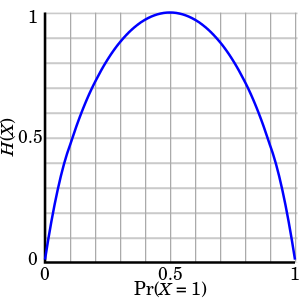
\includegraphics[width=3cm]{bernoulli.png}
    \end{center}
  \end{exampleblock}
\end{frame}

\begin{frame}
  \frametitle{Examples}
  \begin{exampleblock}{Entropy of an unfair dice}
    An unfair dice with four faces and \[ p(1) = 1/2, p(2) = 1/4, p(3) = 1/8, p(4) = 1/8 \] has entropy $7/4$, smaller than the one of the corresponding fair dice, which is $2$. (This dice is less uncertain than the fair dice.)
  \end{exampleblock}
\end{frame}

\begin{frame}
  \frametitle{Motivation: quantifying \emph{information}}
  Define an information function, $I$, in terms of an event $i$ with probability $p_i$, as follows: \pause
  \begin{enumerate}
    \item $I(p)$ is continuous and decreasing \pause
    \item $I(p) \ge 0$ and $I(1) = 0$ \pause
    \item $I(p_1p_2) = I(p_1) + I(p_2)$, i.e. information due to independent events is additive \pause
  \end{enumerate}
  This is solved by $I(p) = - \log p$, up to the base of the logarithm. \pause

  Now, suppose we have a distribution $X$, and we sample it $N$ times. The total amount of information we receive is $\sum N p_i I(p_i)$, and on average, we have $- \sum p_i \log p_i$.
\end{frame}

\begin{frame}
  \frametitle{Joint entropy, conditional entropy}
  \begin{block}{Joint entropy}
    The joint entropy $H(X, Y)$ of a pair of discrete random variables is \[ - \sum \sum p(x, y) \log p(x, y). \]
  \end{block} \pause

  \begin{block}{Conditional entropy}
    The conditional entropy $H(Y|X)$ is defined as \[ \sum p(x) H(Y | X = x). \] \pause
    From this definition, we can derive $H(Y|X) = H(X, Y) - H(X)$.
  \end{block}
\end{frame}

\begin{frame}
  \frametitle{Properties (TPM 15.7.1)}
  \begin{enumerate}
    \item $H(X) \le \log |S|$. \pause
    \item $H(X) \le H(X, Y) \le H(X) + H(Y)$. \pause
    \item $H(X|Y, Z) \le H(X|Y)$. \pause
  \end{enumerate}

  \begin{block}{Entropy is subadditive (TPM 15.7.2)}
    Let $X = (X_1, \dotsc, X_n)$ be a random variable taking values in the set $S = S_1 \times S_2 \times \dotsb \times S_n$, where each of the coordinates $X_i$ of $X$ is a random variable taking values in $S_i$. Then \[ H(X) \le \sum_{i = 1}^n H(X_i). \] \pause (This is just induction on the property $H(X, Y) \le H(X) + H(Y)$.)
  \end{block}
\end{frame}

\begin{frame}
  \frametitle{TPM 15.7.3}
  Let $S$ be a family of subsets of $\{ 1, 2, \dotsc, n \}$ and let $p_i$ denote the fraction of sets in $S$ that contain $i$. Then \[ |S| \le 2^{\sum H(p_i)}. \] \pause

  \begin{block}{Proof}
    Let $X = (X_1, \dotsc, X_n)$ take elements in $S$ with equal probability. Then $H(X) \le \sum H(X_i)$ implies $\log |S| \le \sum H(p_i)$.
  \end{block}
\end{frame}

\begin{frame}
  \frametitle{TPM 15.7.4}
  Let $X = (X_1, \dotsc, X_n)$ taking values in $S = S_1 \times \dotsb \times S_n$, where each $X_i$ takes values in $S_i$. For an index set $I \subseteq N = \{ 1, 2, \dotsc, n \}$ let $X(I)$ denote $(X_i)_{i \in I}$. If $T$ is a family of subsets of $N$ and each $i \in N$ belongs to at least $k$ members of $T$, then \[ kH(X) \le \sum_{G \in T} H(X(G)). \] \pause

  \begin{block}{Proof}
    Use induction. If there is $G \in S$ where $G = N$ we are done. Otherwise, we prove \[ H(X(G \cup G')) + H(X(G \cap G')) \le H(X(G)) + H(X(G')). \]
  \end{block}
\end{frame}

\begin{frame}
  \frametitle{TPM 15.7.5}
  Take $F \subseteq S_1 \times S_2 \times \dotsb \times S_n$. Let $\mathcal{I} = \{ I_1, I_2, \dotsc, I_m \}$ be a collection of index sets (i.e. subsets of $N$), and suppose that each element $i \in N$ belongs to at least $k$ members of $\mathcal{I}$. For each $1 \le i \le m$ let $F_i$ be the set of all projections of the members of $F$ on $I_i$. Then \[ |F|^k \le \prod_{i = 1}^m |F_i|. \] \pause

  \begin{block}{Proof}
    Let $X = (X_1, \dotsc, X_n)$ take elements of $F$ with equal probability. Then $kH(X) \le \sum H(X(I_i))$ implies $k \log |F| \le \sum \log |F_i|$.
  \end{block}
\end{frame}

\begin{frame}
  \frametitle{Corollaries of TPM 15.7.5}
  Take $I_i = N - \{ i \}$ for all $i$, and notice that the volume of a set can be approximated by a collection of fine enough aligned boxes.
  \begin{block}{TPM 15.7.6}
    Let $B$ be a measurable body in the $n$-dimensional Euclidean space, let $Vol(B)$ denote its ($n$-dimensional) volume, and let $Vol(B_i)$ denote the $(n - 1)$-dimensional volume of the projection of $B$ on the hyperplane spanned by all coordinates besides the $i$-th one. Then \[ (Vol(B))^{n - 1} \le \prod_{i = 1}^n Vol(B_i). \]
  \end{block}
\end{frame}

\begin{frame}
  \frametitle{Corollaries of TPM 15.7.5}
  Take $S_i = \{ 0, 1 \}$ in TPM 15.7.5.
  \begin{block}{TPM 15.7.7}
    Let $F$ and $\mathcal{I} = \{ I_1, I_2, \dotsc, I_m \}$ be a collection of subsets of $N$. Suppose that each element of $N$ belongs to at least $k$ members of $\mathcal{I}$. For each $1 \le i \le m$, define $F_i = \{ f \cap I_i : f \in F \}.$ Then \[ |F|^k \le \prod_{i = 1}^m |F_i|. \]
  \end{block}
\end{frame}

\begin{frame}
  \frametitle{Corollaries of TPM 15.7.5}
  \begin{block}{TPM 15.7.8}
    Let $F$ be a family of graphs on the labeled set of vertices $\{ 1, \dotsc, t \}$, and suppose that for any two members of $F$ there is a triangle contained in both of them. Then \[ |F| < \frac{1}{4} 2^{\binom{t}{2}}. \]
  \end{block} \pause

  \begin{block}{Proof}
    Take $N$ to be the set of all edges of $K_t$ and $\mathcal{I}$ be edges of all possible $K_{\lf \frac{t}{2} \rf} \cup K_{\lc \frac{t}{2} \rc}$.
  \end{block}
\end{frame}
\end{document}
